
\begin{figure}[ht]
  \centering
  \begin{subfigure}[t]{0.3\textwidth}
    \centering
    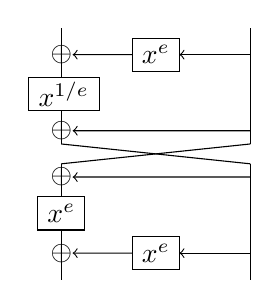
\begin{tikzpicture}[xscale=0.6, yscale=0.42]
      % TOP PART
      % -- cube
      \draw (-0.5, +2.5) rectangle node[pos=0.5]{$x^e$} (+0.5, +3.5);
      % -- cube inverse
      \draw (-1.2, +1.3) rectangle node[pos=0.5]{$x^{1/e}$} (-2.7, +2.3);
      % -- XORs
      \draw (-2.0, +3.0) node[inner sep=0](xor0){$\oplus$} ;
      \draw (-2.0, +0.7) node[inner sep=0](xor1){$\oplus$} ;
      % -- wires
      \draw (+2.0, +3.8) -- (+2.0, +0.3);
      \draw (-2.0, +3.8) -- (-2.0, +2.3);
      \draw[->] (+2.0, +3.0) -- (+0.5, +3.0);
      \draw[->] (-0.5, +3.0) -- (xor0);
      \draw[->] (+2.0, +0.7) -- (xor1);
      \draw (-2.0, +1.3) -- (-2.0, +0.3);
      % MIDDLE WIRING
      \draw (+2.0, +0.3) -- (-2.0, -0.3);
      \draw (-2.0, +0.3) -- (+2.0, -0.3);
      % BOTTOM PART
      % -- cube (xored)
      \draw (-0.5, -2.5) rectangle node[pos=0.5]{$x^e$} (+0.5, -3.5);
      % -- cube
      \draw (-1.5, -1.3) rectangle node[pos=0.5]{$x^{e}$} (-2.5, -2.3);
      % -- XORs
      \draw (-2.0, -3.0) node[inner sep=0](xor2){$\oplus$} ;
      \draw (-2.0, -0.7) node[inner sep=0](xor3){$\oplus$} ;
      % -- wires
      \draw (+2.0, -3.8) -- (+2.0, -0.3);
      \draw (-2.0, -3.8) -- (-2.0, -2.3);
      \draw[->] (+2.0, -3.0) -- (+0.5, -3.0);
      \draw[->] (-0.5, -3.0) -- (xor2);
      \draw[->] (+2.0, -0.7) -- (xor3);
      \draw (-2.0, -1.3) -- (-2.0, -0.3);
    \end{tikzpicture}  
    \FigDef{feistel-ob}{Open butterfly $\openB{e}{1}$}
  \end{subfigure}
  \hspace{0.2cm}
  \begin{subfigure}[t]{0.3\textwidth}
    \centering
    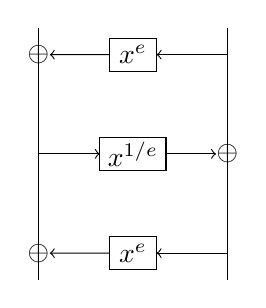
\begin{tikzpicture}[xscale=0.6, yscale=0.42]
      % WIRES
      \draw (+2.0, +3.8) -- (+2.0, -3.8);
      \draw (-2.0, +3.8) -- (-2.0, -3.8);
      % TOP PART
      \draw (-0.5, +2.5) rectangle node[pos=0.5]{$x^e$} (+0.5, +3.5);
      \draw (-2.0, +3.0) node[inner sep=0](xor0){$\oplus$} ;
      \draw[->] (+2.0, +3.0) -- (+0.5, +3.0);
      \draw[->] (-0.5, +3.0) -- (xor0);
      % MIDDLE PART
      \draw (-0.7, -0.5) rectangle node[pos=0.5]{$x^{1/e}$} (+0.7, +0.5);
      \draw (+2.0, +0.0) node[inner sep=0](xor1){$\oplus$} ;
      \draw[->] (-2.0, +0.0) -- (-0.7, +0.0);
      \draw[->] (+0.7, +0.0) -- (xor1);
      % BOTTOM PART
      \draw (-0.5, -2.5) rectangle node[pos=0.5]{$x^e$} (+0.5, -3.5);
      \draw (-2.0, -3.0) node[inner sep=0](xor2){$\oplus$} ;
      \draw[->] (+2.0, -3.0) -- (+0.5, -3.0);
      \draw[->] (-0.5, -3.0) -- (xor2);
    \end{tikzpicture}  
    \FigDef{feistel-fn}{$\feistelB{e} = \openB{e}{1}$}
  \end{subfigure}
  \hspace{0.2cm}
  \begin{subfigure}[t]{0.3\textwidth}
    \centering
    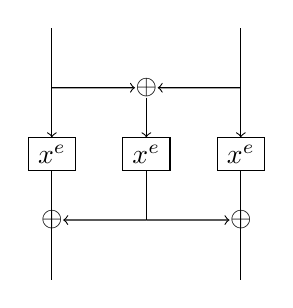
\begin{tikzpicture}[xscale=0.6, yscale=0.42]
      % S-BOX LAYER
      \draw (-2.5, -0.5) rectangle node[pos=0.5]{$x^e$} (-1.5, +0.5);
      \draw (-0.5, -0.5) rectangle node[pos=0.5]{$x^e$} (+0.5, +0.5);
      \draw (+1.5, -0.5) rectangle node[pos=0.5]{$x^e$} (+2.5, +0.5);
      % WIRES
      \draw[->] (+2.0, +3.8) -- (+2.0, +0.5);
      \draw[->] (-2.0, +3.8) -- (-2.0, +0.5);
      \draw (+2.0, -0.5) -- (+2.0, -3.8);
      \draw (-2.0, -0.5) -- (-2.0, -3.8);
      % XORS
      \draw (+0.0, +2.0) node[inner sep=0](xorTop){$\oplus$} ;
      \draw (+2.0, -2.0) node[inner sep=0](xorLeft){$\oplus$} ;
      \draw (-2.0, -2.0) node[inner sep=0](xorRight){$\oplus$} ;
      \draw[->] (-2.0, +2.0) -- (xorTop);
      \draw[->] (+2.0, +2.0) -- (xorTop);
      \draw[->] (xorTop) -- (+0.0, +0.5);
      \draw (+0.0, -0.5) -- (+0.0, -2.0);
      \draw[->] (+0.0, -2.0) -- (xorLeft);
      \draw[->] (+0.0, -2.0) -- (xorRight);
    \end{tikzpicture}  
    \FigDef{feistel-lm}{Closed butterfly $\closedB{e}{1}$}
  \end{subfigure}
  \FigDef{feistel}{The equivalence between $\openB{e}{1}$ and $\feistelB{e}$.}
\end{figure}